%%%%%%%%%%%%%%%%%%%%%%%%%%%%%%%%%%%%%%%%%%%%%%%%%%%%%%%%%%%%%%%%%%%%%%%%%%%%%%%%%%%%%%%%%%%%%%%%
%
% CS484 Written Question Template
%
% Acknowledgements:
% The original code is written by Prof. James Tompkin (james_tompkin@brown.edu).
% The second version is revised by Prof. Min H. Kim (minhkim@kaist.ac.kr).
%
% This is a LaTeX document. LaTeX is a markup language for producing 
% documents. Your task is to fill out this document, then to compile 
% it into a PDF document. 
%
% 
% TO COMPILE:
% > pdflatex thisfile.tex
%
% If you do not have LaTeX and need a LaTeX distribution:
% - Personal laptops (all common OS): www.latex-project.org/get/
% - We recommend latex compiler miktex (https://miktex.org/) for windows,
%   macTex (http://www.tug.org/mactex/) for macOS users.
%   And TeXstudio(http://www.texstudio.org/) for latex editor.
%   You should install both compiler and editor for editing latex.
%   The another option is Overleaf (https://www.overleaf.com/) which is 
%   an online latex editor.
%
% If you need help with LaTeX, please come to office hours. 
% Or, there is plenty of help online:
% https://en.wikibooks.org/wiki/LaTeX
%
% Good luck!
% Min and the CS484 staff
%
%%%%%%%%%%%%%%%%%%%%%%%%%%%%%%%%%%%%%%%%%%%%%%%%%%%%%%%%%%%%%%%%%%%%%%%%%%%%%%%%%%%%%%%%%%%%%%%%
%
% How to include two graphics on the same line:
% 
% \includegraphics[\width=0.49\linewidth]{yourgraphic1.png}
% \includegraphics[\width=0.49\linewidth]{yourgraphic2.png}
%
% How to include equations:
%
% \begin{equation}
% y = mx+c
% \end{equation}
% 
%%%%%%%%%%%%%%%%%%%%%%%%%%%%%%%%%%%%%%%%%%%%%%%%%%%%%%%%%%%%%%%%%%%%%%%%%%%%%%%%%%%%%%%%%%%%%%%%

\documentclass[11pt]{article}

\usepackage[english]{babel}
\usepackage[utf8]{inputenc}
\usepackage[colorlinks = true,
            linkcolor = blue,
            urlcolor  = blue]{hyperref}
\usepackage[a4paper,margin=1.5in]{geometry}
\usepackage{stackengine,graphicx}
\usepackage{fancyhdr}
\setlength{\headheight}{15pt}
\usepackage{microtype}
\usepackage{times}
\usepackage{booktabs}
\usepackage{amsmath}
\usepackage[export]{adjustbox}
\usepackage{longtable}

% From https://ctan.org/pkg/matlab-prettifier
\usepackage[numbered,framed]{matlab-prettifier}

\frenchspacing
\setlength{\parindent}{0cm} % Default is 15pt.
\setlength{\parskip}{0.3cm plus1mm minus1mm}

\pagestyle{fancy}
\fancyhf{}
\lhead{Homework Writeup}
\rhead{CS484}
\rfoot{\thepage}

\date{}

\title{\vspace{-1cm}Homework 3 Writeup}


\begin{document}
\maketitle
\vspace{-3cm}
\thispagestyle{fancy}

\section*{Instructions}
\begin{itemize}
  \item Describe any interesting decisions you made to write your algorithm.
  \item Show and discuss the results of your algorithm.
  \item Feel free to include code snippets, images, and equations.
  \item Use as many pages as you need, but err on the short side If you feel you only need to write a short amount to meet the brief, th
  
  \item \textbf{Please make this document anonymous.}
\end{itemize}

\section*{Algorithm Implementation}

The implementation of the stereo imaging is divided into four parts.
\subsection{Bayer Image Interpolation}
To convert the Bayer image into an RGB version, bicubic interpolation was used. Shortened code is shown below, please refer to the \emph{bayer\_to\_rgb\_bicubic.m} file for the full version. In lines up to 8, the Bayer image is separated into four channels of R,G1,G2 and B. The G channel is divided into G1 and G2 because bicubic interpolation uses 16 nearest known colors, but it was difficult to choose 16 nearest points from the layout of the G channel. So G1 and G2 were considered as two separate channels. They were later combined to form a single channel G in lines 10 to 17. In the function \emph{bicubic}, bicubic interpolation of the input channel is implemented as described in \href{http://www.ahinson.com/algorithms_general/Sections/InterpolationRegression/InterpolationBicubic.pdf}{InterpolationBicubic.pdf}. The channel is first padded appropriately by repeating the border pixels. Then I found matrices \emph{X}, \emph{Y}, \emph{Z}, \emph{Px} and \emph{Py} one by one. \emph{X} and \emph{Y} are offset arrays in x and y directions, respectively. \emph{Z} is the array of values of nearest 16 pixels. \emph{Px} and \emph{Py} are the arrays of normalized distance to the nearest pixels, raised to up to the third power. For each \emph{(i,j)} of channel, the distance to the nearest upper left pixel was used to find \emph{Z},  \emph{Px} and \emph{Py}. The result of interpolation can be expressed as $[Py][Y^{-1}][Z][X^{-1}][Px]$. An interesting point is that if the commented matrix in line 33 for the offset matrix \emph{X} is used instead of the original one, the resulting image looks more natural. The comparison is discussed in the results section (Figure~\ref{fig:x_comparison}).

\begin{lstlisting}[style=Matlab-editor]
function rgb_img = bayer_to_rgb_bicubic(bayer_img)
    ...
    window=["r", "g1"; "g2", "b"];
    repWindow=repmat(window, img_size/2);
    r_channel(repWindow=="r")=bayer_img(repWindow=="r");
    g1_channel(repWindow=="g1")=bayer_img(repWindow=="g1");
    g2_channel(repWindow=="g2")=bayer_img(repWindow=="g2");
    b_channel(repWindow=="b")=bayer_img(repWindow=="b");
    r=bicubic(r_channel);
    g1=rot90(bicubic(rot90(g1_channel)),3);
    g2=rot90(bicubic(rot90(g2_channel,3)));
    g=zeros(size(g1));
    avgg=(g1+g2)/2;
    g((repWindow=='b'))=avgg(repWindow=='b');
    g((repWindow=='r'))=avgg(repWindow=='r');
    g((repWindow=='g1'))=g1_channel(repWindow=='g1');
    g((repWindow=='g2'))=g2_channel(repWindow=='g2');
    b=rot90(bicubic(rot90(b_channel,2)),2);
    rgb_img=uint8(cat(3,r,g,b));
    ...
end

function result = bicubic(channel)
    padded=cat(1, channel(1:2,:), channel);
    padded=cat(1,padded, padded(size(padded,1)-1:size(padded,1),:));
    padded=cat(1,padded, padded(size(padded,1)-1,:));
    padded=cat(2,padded(:,1:2), padded);
    padded=cat(2, padded, padded(:,size(padded,2)-1:size(padded,2)));
    padded=cat(2, padded, padded(:,size(padded,2)-1));
    paddedCpy=padded;

    X=[-1 0 1 8; 1 0 1 4; -1 0 1 2; 1 1 1 1];
%    X=[-8 0 8 64; 4 0 4 16; -2 0 2 4; 1 1 1 1];
    Y=X';
    for i=3:size(padded,1)-3
        for j=3:size(padded,2)-3
            if padded(i,j)==0
                d=normalizedDistance(i,j);
                centerP=[i j]-d;
                Z=reshape(nonzeros(padded(centerP(1)-2:centerP(1)+4,centerP(2)-2:centerP(2)+4)),4,4);
                px=[d(1)^3; d(1)^2; d(1); 1];
                py=[d(2)^3 d(2)^2 d(2) 1];
                p=py*inv(Y)*Z*inv(X)*px;
                paddedCpy(i,j)=p;
            end
        end
    end
    result=paddedCpy(3:size(padded,1)-3,3:size(padded,2)-3);
end

function n=normalizedDistance(i,j)
    n=[0 0];
    if mod(i,2)==0
        n(1)=1;
    else
        n(1)=0;
    end
    if mod(j,2)==0
        n(2)=1;
    else
        n(2)=0;
    end
end


\end{lstlisting}

\subsection{Fundamental Matrix Calculation}
The fundamental matrix is calculated using the eight-point algorithm. Full code shown below. First, the matching points are normalized in lines 3 to 4. Then, the A matrix of the eight point algorithm formula $Af=0$ is constructed in lines 10 to 12. The fundamental matrix F is initially made by reshaping the eigenvector corresponding to the smallest eigenvalue of $A^TA$. This is done in line 13. This is part of the least squares approach. Then, F is updated by changing the smallest eigenvalue to 0. This is done in line 14. Because this is a normalized eight point algorithm, the fundamental matrix should be turned back into original units. This is done in line 16.

\begin{lstlisting}[style=Matlab-editor]
function f = calculate_fundamental_matrix(pts1, pts2)
    clc;
    [pts1, T1]=normalize_points(pts1', 2);
    [pts2, T2]=normalize_points(pts2', 2);
    pts1=pts1';
    pts2=pts2';
    x=padarray(pts1',1,1,'post');
    xp=padarray(pts2,[0 1],1,'post');
    A=[];
    for i=1:size(x,2)
        A=cat(1,A,reshape((x(:,i).*xp(i,:))',[1 9]));
    end
    F=reshape(smallest_eigenvector(A'*A),[3 3])
    F=update_sv(F)
    
    f = T2'*F*T1
end

function v = smallest_eigenvector(A)
    [V,D] = eig(A);
    [d,ind] = sort(diag(D));
    Ds = D(ind,ind);
    Vs = V(:,ind);
    v=Vs(:,1);
end

function Fp = update_sv(F)
    [U,S,V]=svd(F);
    [~,idx]=sort(diag(S));
    S=S(idx, idx);
    V=V(:,idx);
    U=U(:,idx);
    S(1,1)=0;
    Fp=U*S*V';
end
\end{lstlisting}


\subsection{Image Rectification}
In this section, the left and right images were rectified using their respective homography matrices. Full code shown below. First, the two homograpy matrices were converted into transformations in lines 3 and 4. Then the four corners of each image was transformed into the space of the final image in lines 9 and 10. But because these points contain negative coordinates, they should be shifted so that they exist in the positive coordinate space. Such shift amount was found in line 13 by finding the minimum values in the corner coordinates. The corners were then shifted in line 14. Then, the images were warped using the transformations in lines 16 and 17. Now the images are transformed into the final image space, but they are not aligned. The amount of offset for alignment of each image can be found from the transformed corners as in lines 21 and 22. They are the minimum values in the respective corner coordinates. The image are translated by the found amount in lines 24 and 25. Then, the size of the aligned image is determined in line 27, which is the maximum of the dimensions of the separate images. Lines 29 and 30 are executed so that the aligned images have the same size (the final image size) by adding appropriate amount of padding. 

\begin{lstlisting}[style=Matlab-editor]
function [rectified1, rectified2] = rectify_stereo_images(img1, img2, h1, h2)

    tform1 = projective2d(h1);
    tform2 = projective2d(h2);
    
    corners1 = [1 1; size(img1,2) 1; 1 size(img1,1); size(img1,2) size(img1,1)]
    corners2 = [1 1; size(img2,2) 1; 1 size(img2,1); size(img2,2) size(img2,1)]
    
    tcorners1 = transformPointsForward(tform1,corners1);
    tcorners2 = transformPointsForward(tform2,corners2);
    tcorners = [tcorners1; tcorners2]
    
    shift = [-min(tcorners(:,1))+1, -min(tcorners(:,2))+1]
    tcorners = tcorners+shift
    
    img1 = imwarp(img1, tform1);
    img2 = imwarp(img2, tform2);
    
    tcorners1 = tcorners1+shift;
    tcorners2 = tcorners2+shift;
    offset1 = [min(tcorners1(:,1))-1 min(tcorners1(:,2))-1]
    offset2 = [min(tcorners2(:,1))-1 min(tcorners2(:,2))-1]
    
    img1 = imtranslate(img1,offset1,'OutputView','full');
    img2 = imtranslate(img2,offset2,'OutputView','full');
    
    max_size = round([max(size(img1,1), size(img2,1)) max(size(img1,2), size(img2,2))])
    
    rectified1 = padarray(img1,[max_size(1)-size(img1,1) max_size(2)-size(img1,2)], 0,'post');
    rectified2 = padarray(img2,[max_size(1)-size(img2,1) max_size(2)-size(img2,2)], 0,'post');
end
\end{lstlisting}
\subsection{Disparity Map Calculation}
The disparity map was created from the aligned images. Different parameters such as the window size, maximum disparity, and filter amount were tested to get the best results. The full code of disparity map calculation is show below. First, an empty cost volume is created in line 3 with size according to the image size and the maximum disparity. Then, each pixel of the left image \emph{(i,j)} is iterated, storing the normalized cross correlation value with the pixel of the right image separated by \emph{k} pixels in \emph{(i,j,k)}. Because we can assume that a corresponding window of the right window exists on the right of it, in other words, the left image exists on the right of the right image, we can improve efficiency by only looking at the windows on the right of the left image located at \emph{(j-k)}, as shown in line 11. Then, for each plane in the cost volume, cost was aggregated using a Gaussian filter and was experimented with varying standard deviation values. The normalized cross correlation was implemented in a separate function. The input matrices A and B were subtracted the mean of each. Then, the cross correlation was calculated according to the formula $\frac{ \sum \sum A(i,j)B(i,j)}{\sqrt{\sum \sum A(i,j)^{2}}\sqrt{\sum \sum B(i,j)^{2}}}$. Because a NaN error occurs if either A or B contains only 0 elements, such cases were avoided by immediately returning 0, thus not altering the cost volume. The comparison of various parameters are discussed in the results section.
\begin{lstlisting}[basicstyle=\ttfamily\tiny, style=Matlab-editor]
function d = calculate_disparity_map(img_left, img_right, window_size, max_disparity)
        
    cost_vol = zeros(size(img_left,1), size(img_left,2), max_disparity);
    size(cost_vol)
    
    for i = ceil(window_size/2):size(img_left,1)-floor(window_size/2)
        for j = ceil(window_size/2):size(img_left,2)-floor(window_size/2)
            l = img_left(i-floor(window_size/2):i+floor(window_size/2),j-floor(window_size/2):j+floor(window_size/2));
            for k = 1:max_disparity
                if (j-k)-floor(window_size/2)>0
                    r = img_right(i-floor(window_size/2):i+floor(window_size/2),(j-k)-floor(window_size/2):(j-k)+floor(window_size/2));
                    cost_vol(i,j,k) = ncc(l,r);
                end
            end
        end
    end
    
    cost_vol = smooth_planes(cost_vol);


    % winner takes all
    [min_val, d] = max(cost_vol,[],3);

end

function c = ncc(A, B)
    A = A-mean(A(:));
    B = B-mean(B(:));
    if nnz(A) == 0 || nnz(B) == 0
        c = 0;
    else
        rA = sqrt(sum(sum(A.^2,1)));
        rB = sqrt(sum(sum(B.^2,1)));
        ab = sum(sum(A.*B,1));
        c = ab/(rA*rB);
    end
end

function vol = smooth_planes(vol)
    for d = 1:size(vol,3)
        vol(:,:,d) = imgaussfilt(vol(:,:,d),1);
    end
end
\end{lstlisting}

\section*{Results}

\subsection{Bayer Image Interpolation}
The figure below shows the matching points of left and right interpolated images.

\begin{figure}[h]
	\centering
	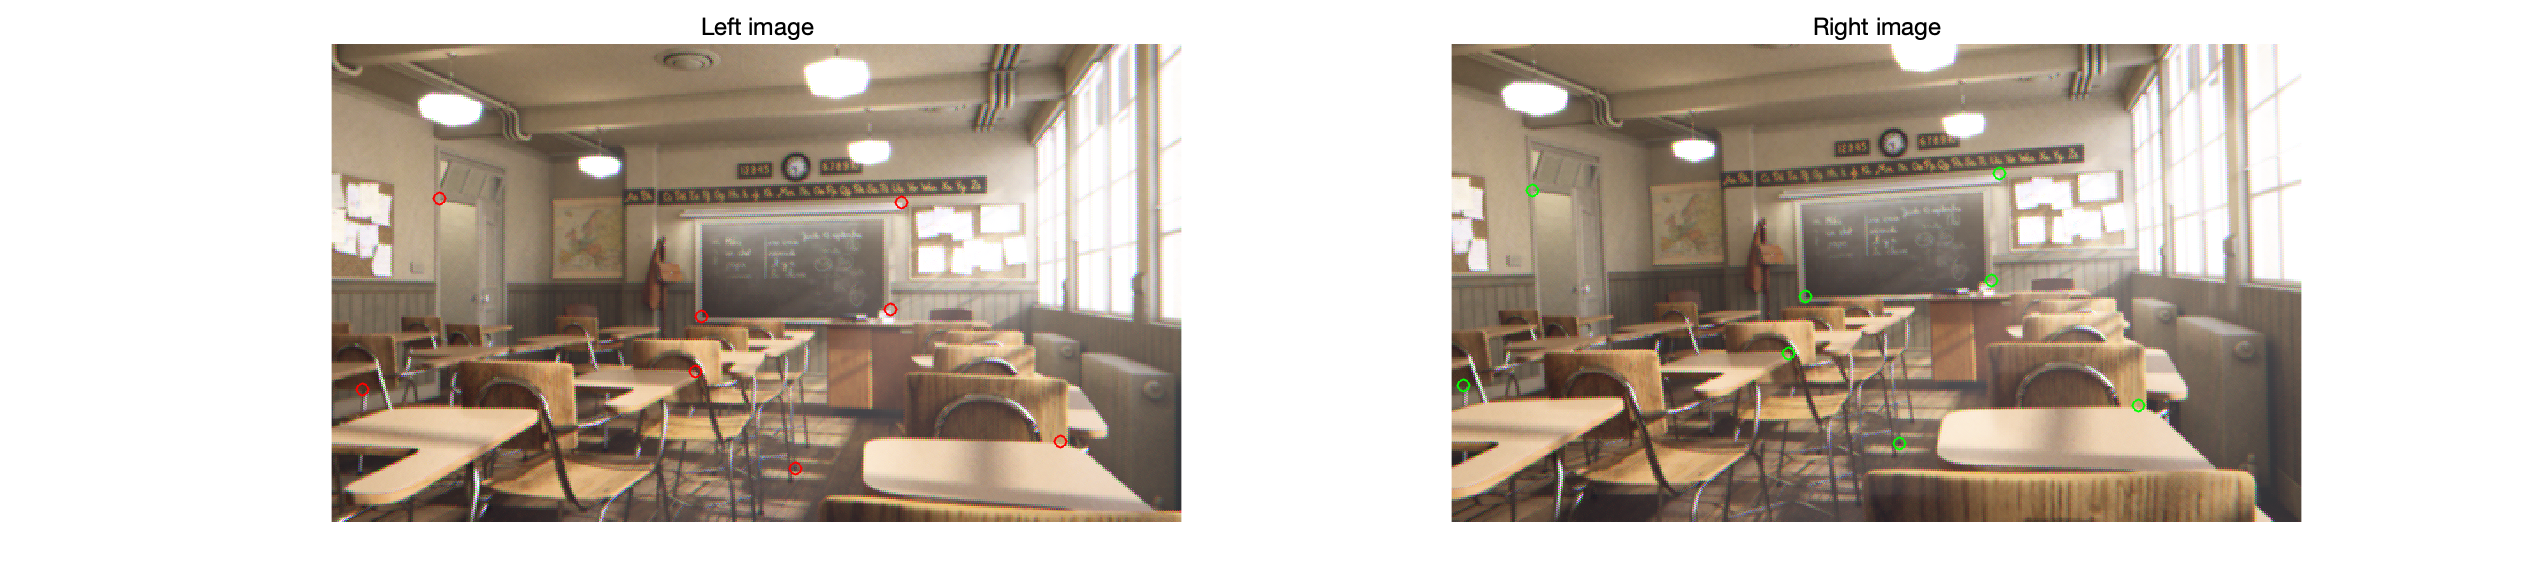
\includegraphics[width=\textwidth]{../code/part1_result.png}
	\caption{Matching points.}
	\label{fig:matching_points}
\end{figure}

Figure~\ref{fig:x_comparison} compares the different values for X. The first image is made by using the correct offset matrix
\[
\begin{bmatrix}
-1       & 0& 1&8 \\
1       & 0 & 1&4 \\
-1       & 0 & 1&2\\
1 & 1 & 1 & 1
\end{bmatrix}
\]
 while the second one used
 \[
 \begin{bmatrix}
 -8       & 0& 8&64 \\
 4       & 0 & 4&16 \\
 -2       & 0 & 2&4\\
 1 & 1 & 1 & 1
 \end{bmatrix}
 \]
 . Using the second option means we use the second-closest 16 points not the closest 16 points. That's why the offsets are mutiples of 2 not 1. Although the second option is not the true bicubic interpolation, it provided somewhat clearer and more natural looking image. As shown in Figure~\ref{fig:x_comparison}, the first one has visible red, green and blue blocks at edges in the image, while the second one does not. The first option was used through later parts but using the second option created no visible differences.

\begin{figure}[h]
    \centering
    \adjincludegraphics[width=0.45\textwidth,trim={0 0 {.8\width} {.6\height}},clip]{../code/first_x_left.png}
    \adjincludegraphics[width=0.45\textwidth,trim={0 0 {.8\width} {.6\height}},clip]{../code/second_x_left.png}
    \caption{\emph{Left:} First X matrix. \emph{Right:} Second X matrix.}
    \label{fig:x_comparison}
\end{figure}

\subsection{Fundamental Matrix Calculation}
The fundamental matrix is calculated as below from the algorithm explained in the implementation section.
\[
\begin{bmatrix}
0       & 0& 0 \\
0       & 0 & 0.0046 \\
0.0002       & -0.0046 & 0.0215
\end{bmatrix}
\]

\subsection{Image Rectification}
Figure~\ref{fig:before_alignment} shows the rectified images before paddings were applied for alignment. After the calculation of the offset, the images were translated by the amount calculated in the algorithm to be aligned. Figure~\ref{fig:rectified} shows the rectified images and their alignment.
\begin{figure}[h!]
	\centering
	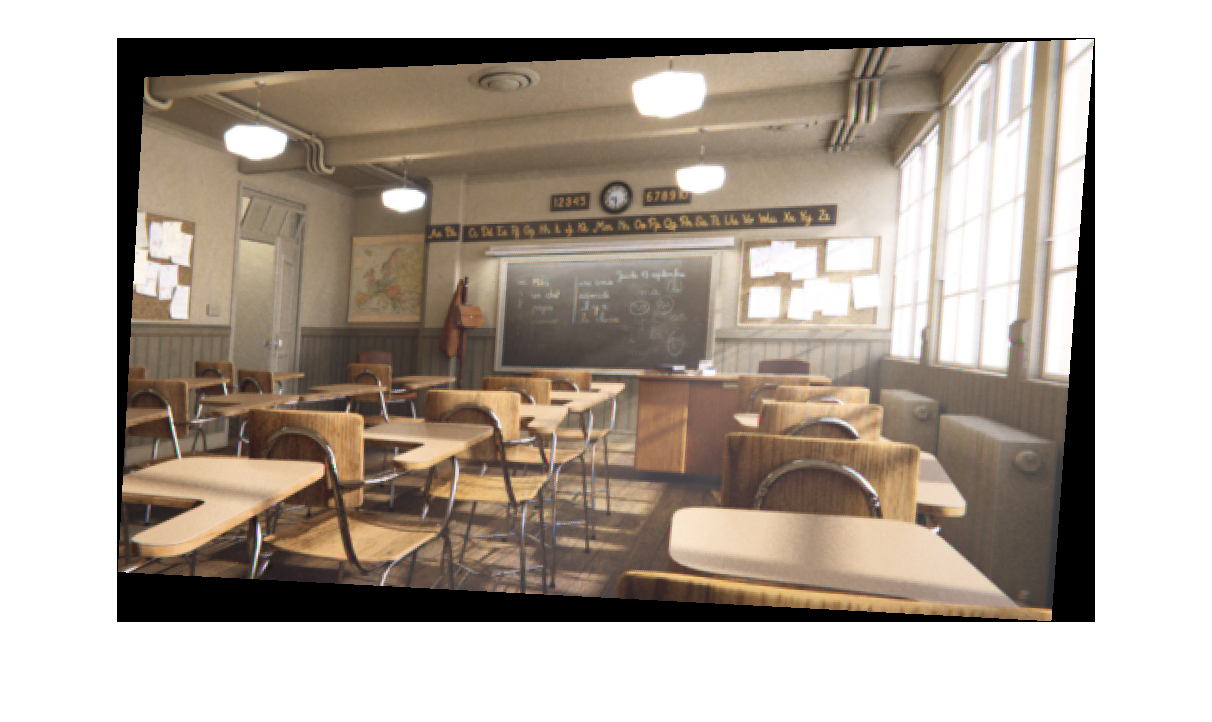
\includegraphics[width=0.45\textwidth]{../code/rectified_left.png}
	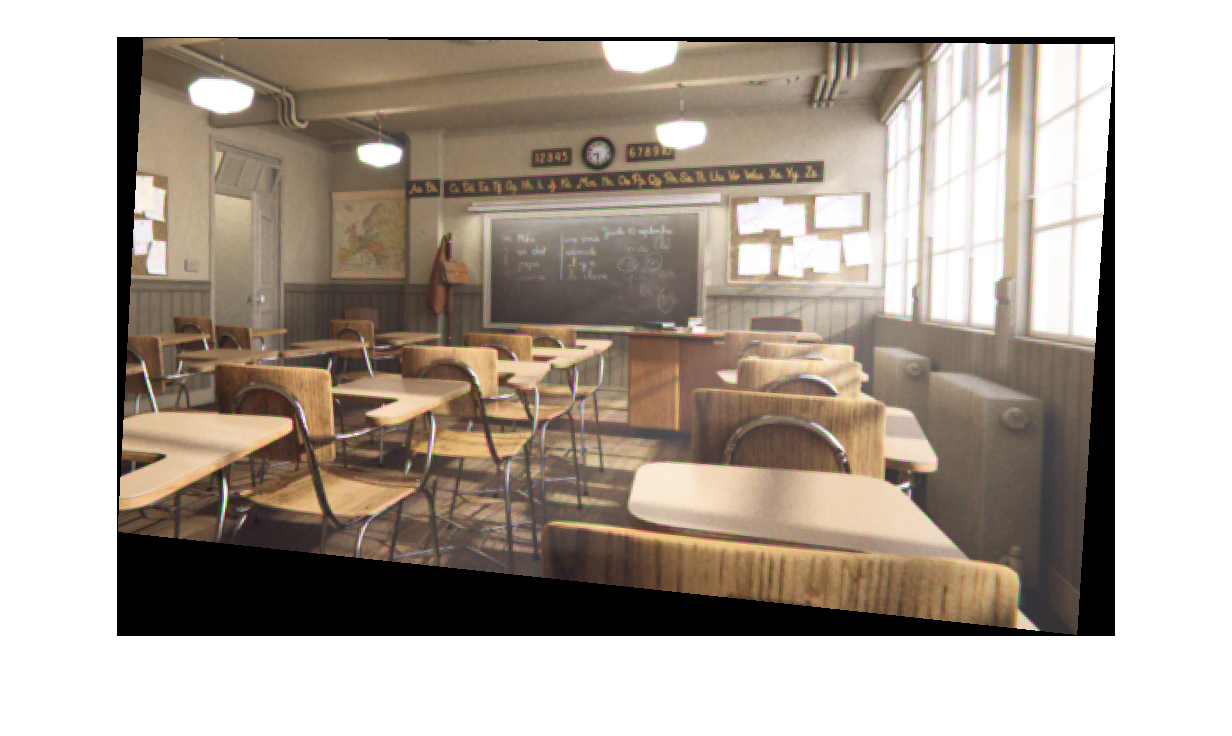
\includegraphics[width=0.45\textwidth]{../code/rectified_right.png}
	\caption{Before alignment.}
	\label{fig:before_alignment}
\end{figure}

\begin{figure}[h!]
	\centering
	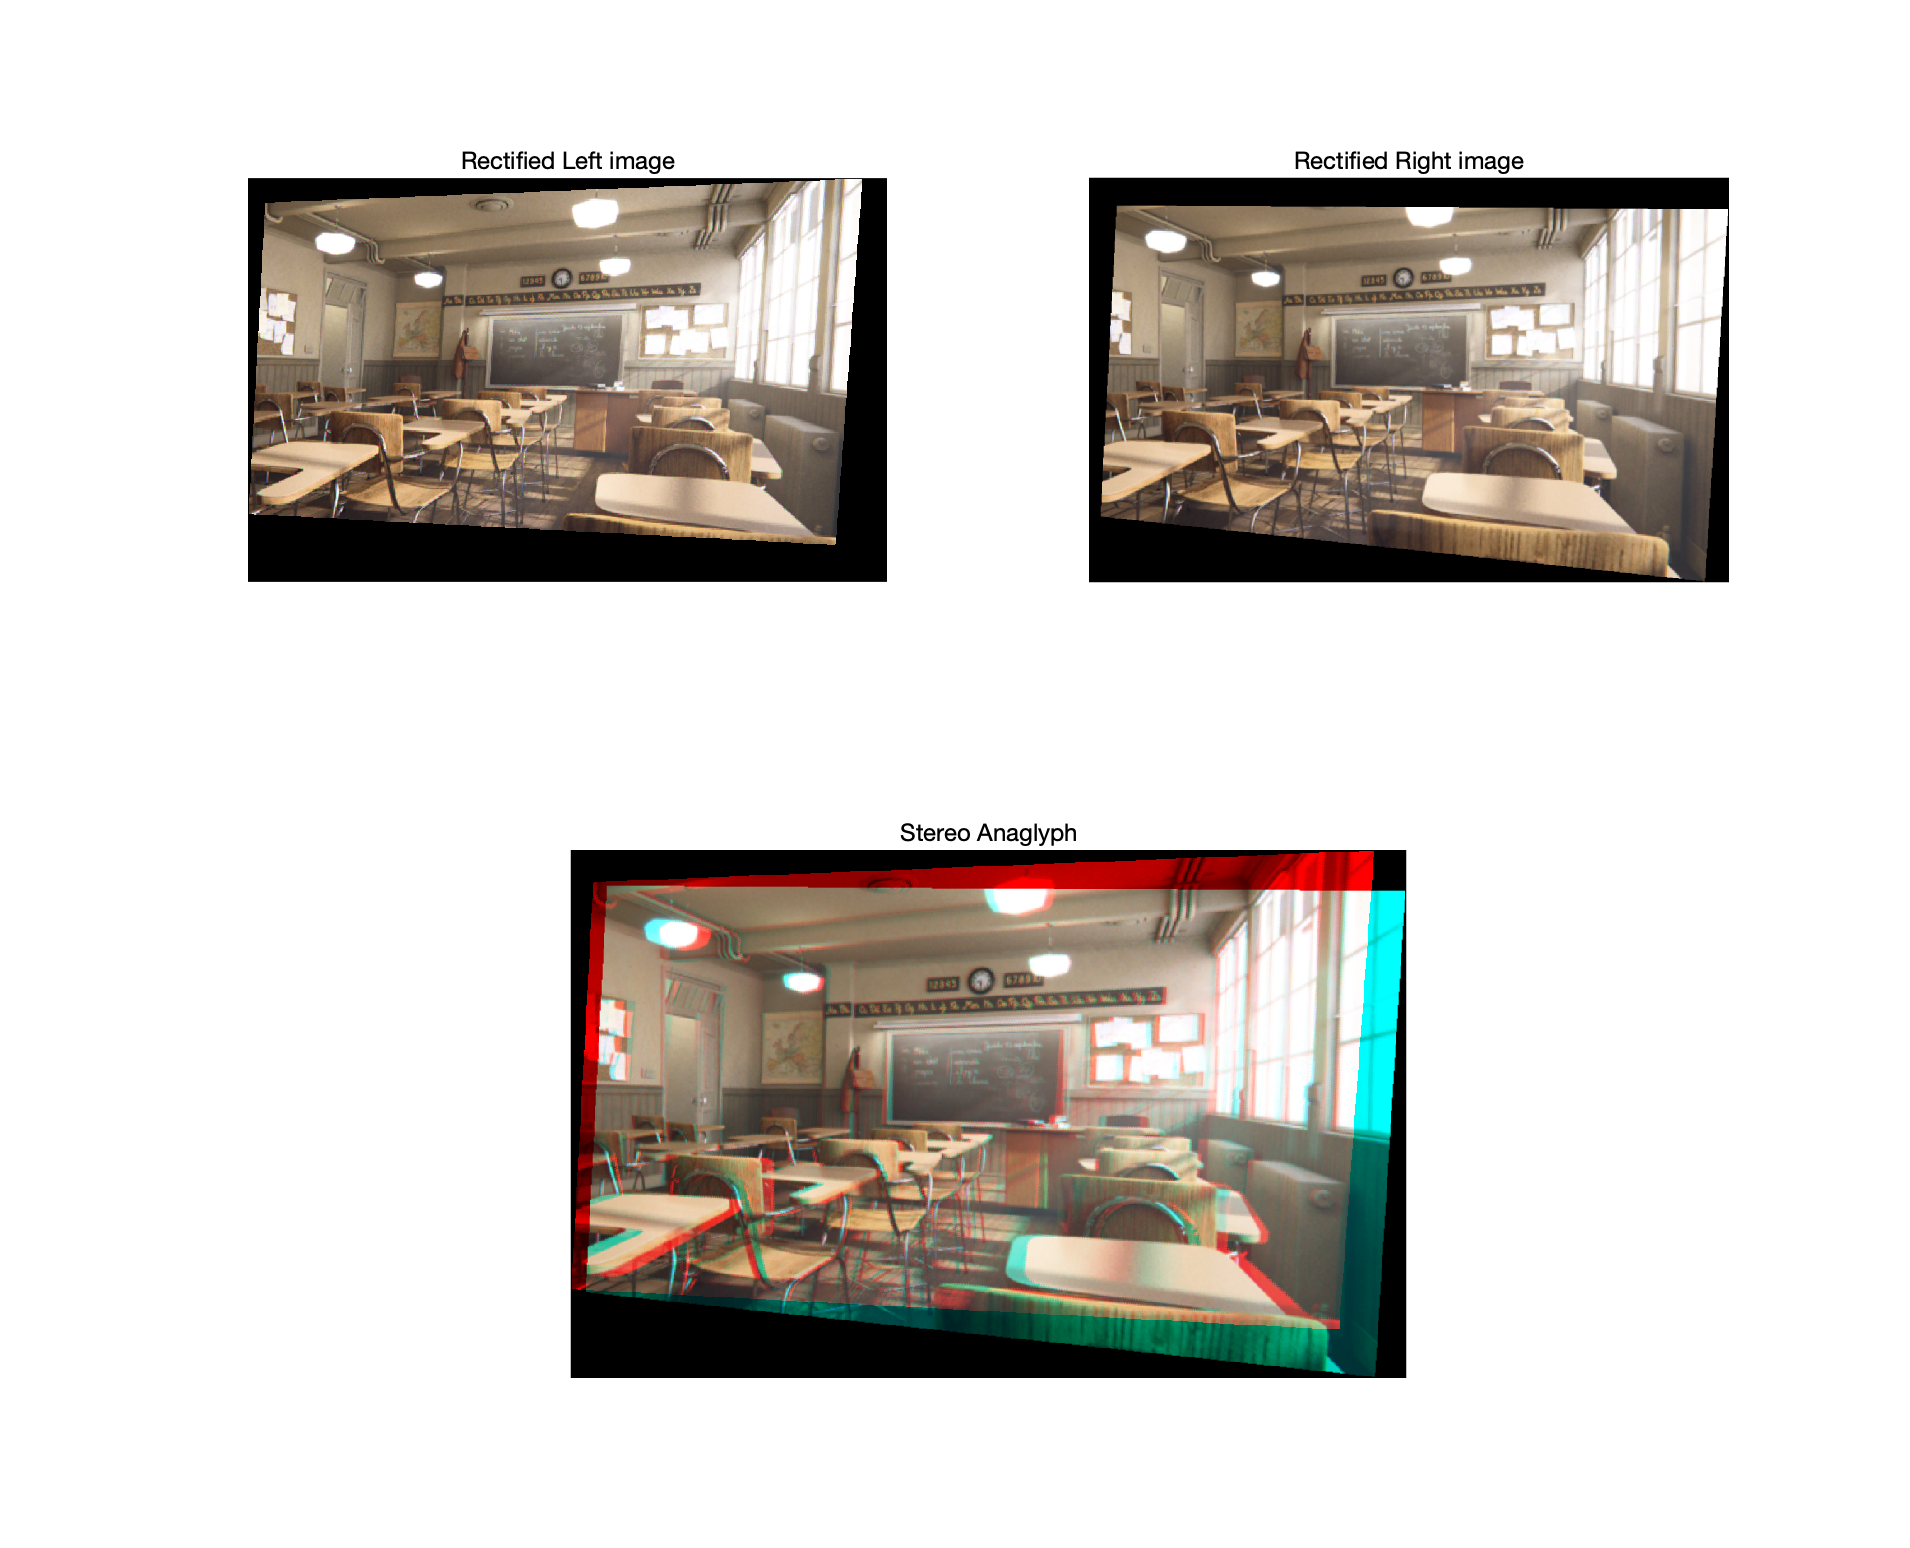
\includegraphics[width=\textwidth]{../code/rectified.png}
	\caption{Rectified images and alignment.}
	\label{fig:rectified}
\end{figure}

\subsection{Disparity Map Calculation}
Table~\ref{tab:table1} shows the comparison of disparity maps created with different parameters. In my opinion, the map created with window size of 5 pixel, standard deviation of 2, and maximum disparity of 40 looks the best. It is shown in Figure~\ref{fig:best_map}. Smaller window size tend to make the map look noisy and larger sigma made the regions rounder in the map. The difference between the maximum disparity of 40 and 60 was not great. Therefore, we can conclude that maximum disparity of 40 was enough to capture all the disparities.

\begin{figure}[h!]
	\centering
	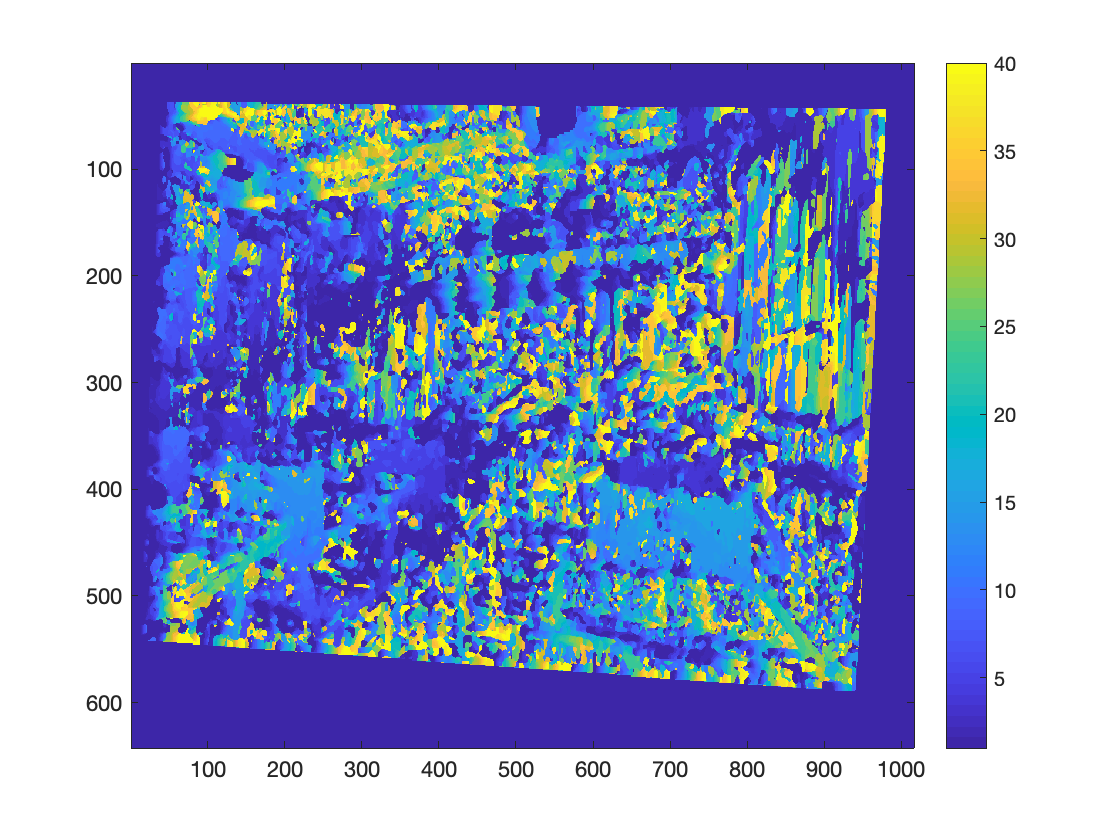
\includegraphics[width=\textwidth]{../code/win5sig2.png}
	\caption{Depth map from 5px window, sigma 2, max disparity 40.}
	\label{fig:best_map}
\end{figure}

\begin{longtable}[h!]{|c|c|}
	\caption{Comparison of different parameters of disparity map.}
	\label{tab:table1}\\
	\hline
	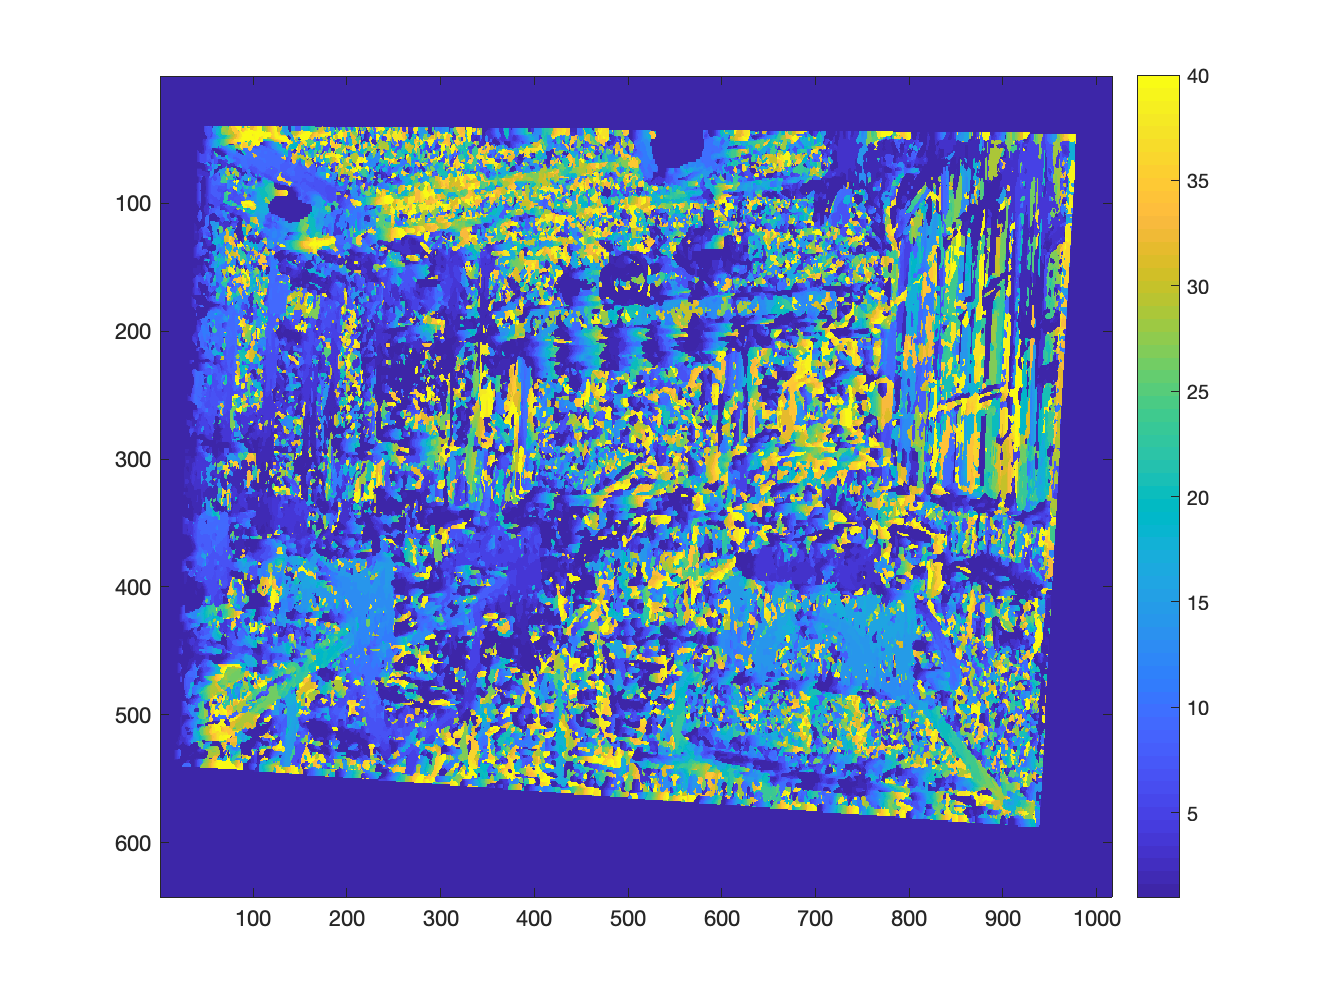
\includegraphics[width=0.4\textwidth]{../code/win5sig1.png} & 
	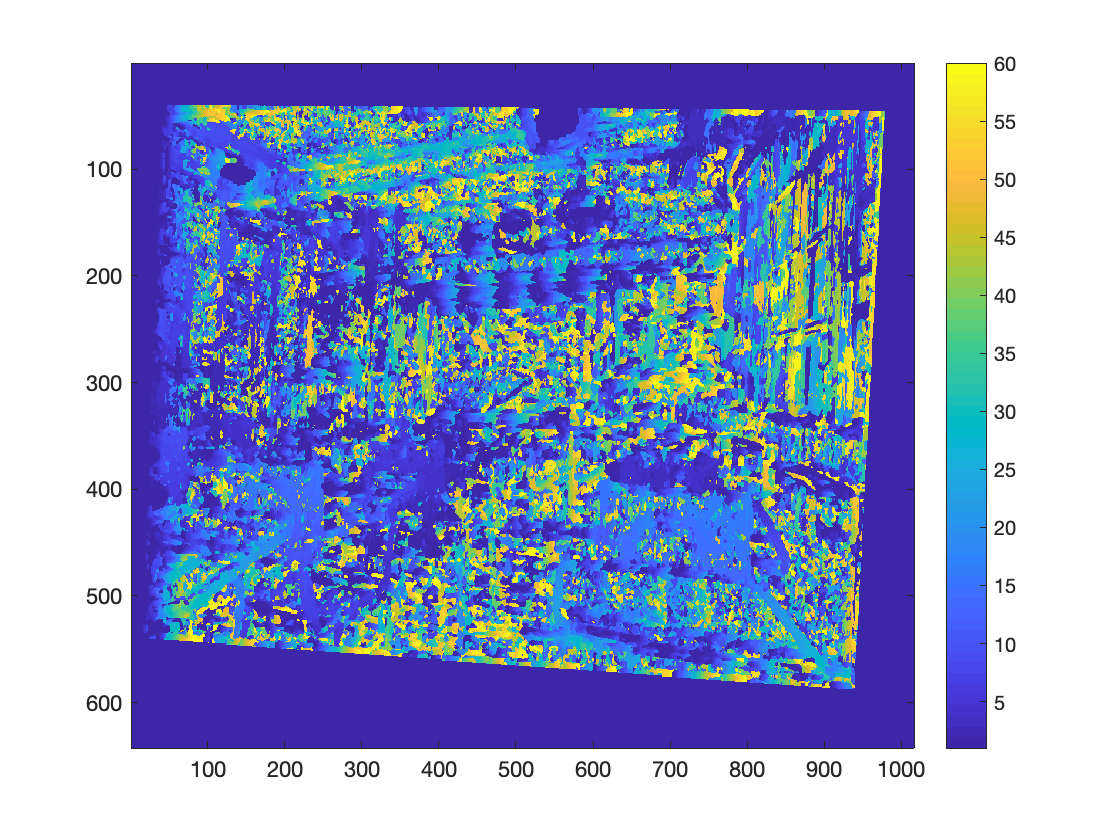
\includegraphics[width=0.4\textwidth]{../code/win5sig1disp60.png} \\
	\hline
	window size:5px, sigma:1, max\_disparity:40 &window size:5px, sigma:1, max\_disparity:60\\
	\hline
	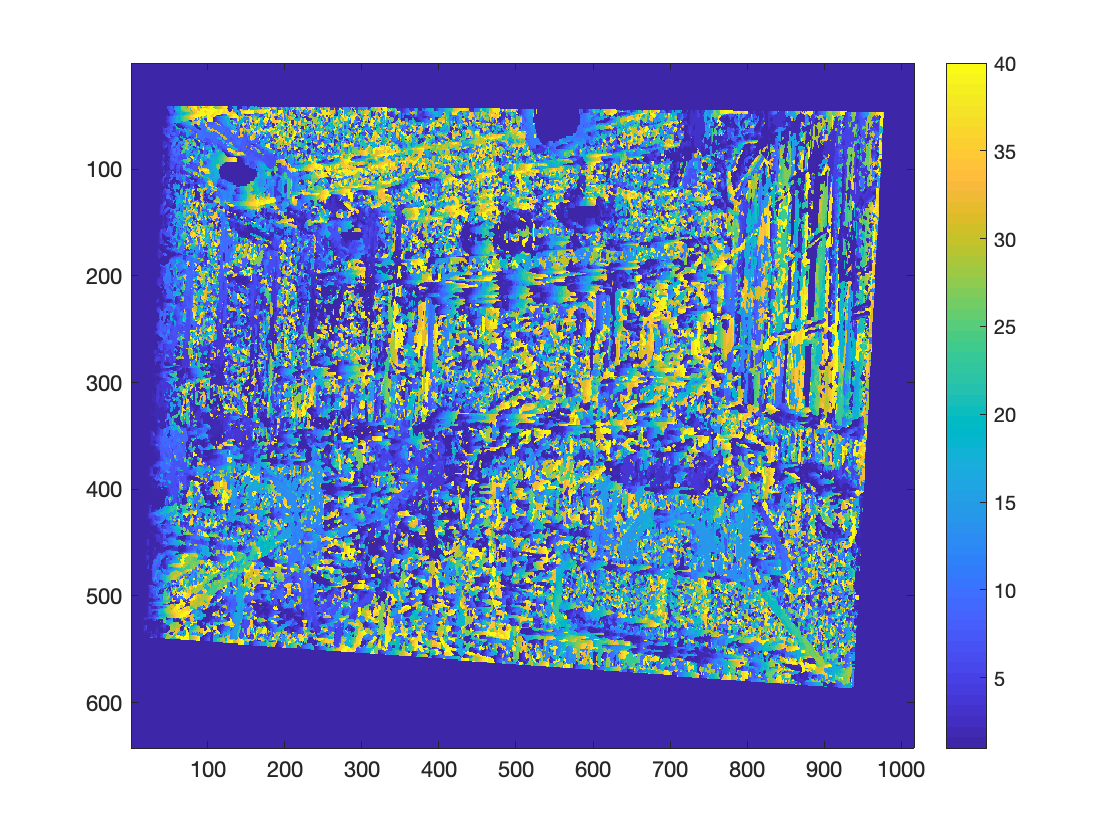
\includegraphics[width=0.4\textwidth]{../code/win3sig1.png} & 
	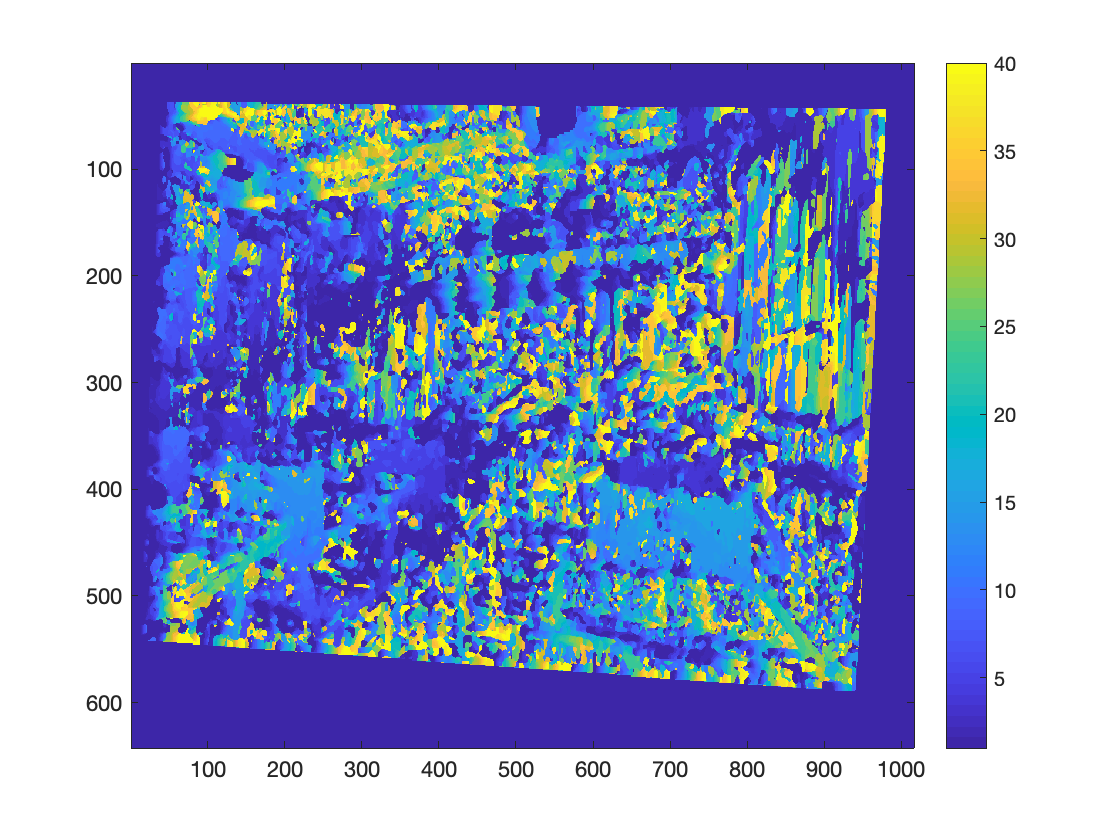
\includegraphics[width=0.4\textwidth]{../code/win5sig2.png} \\
	\hline
	window size:3px, sigma:1, max\_disparity:40 &window size:5px, sigma:2, max\_disparity:40\\
	\hline
	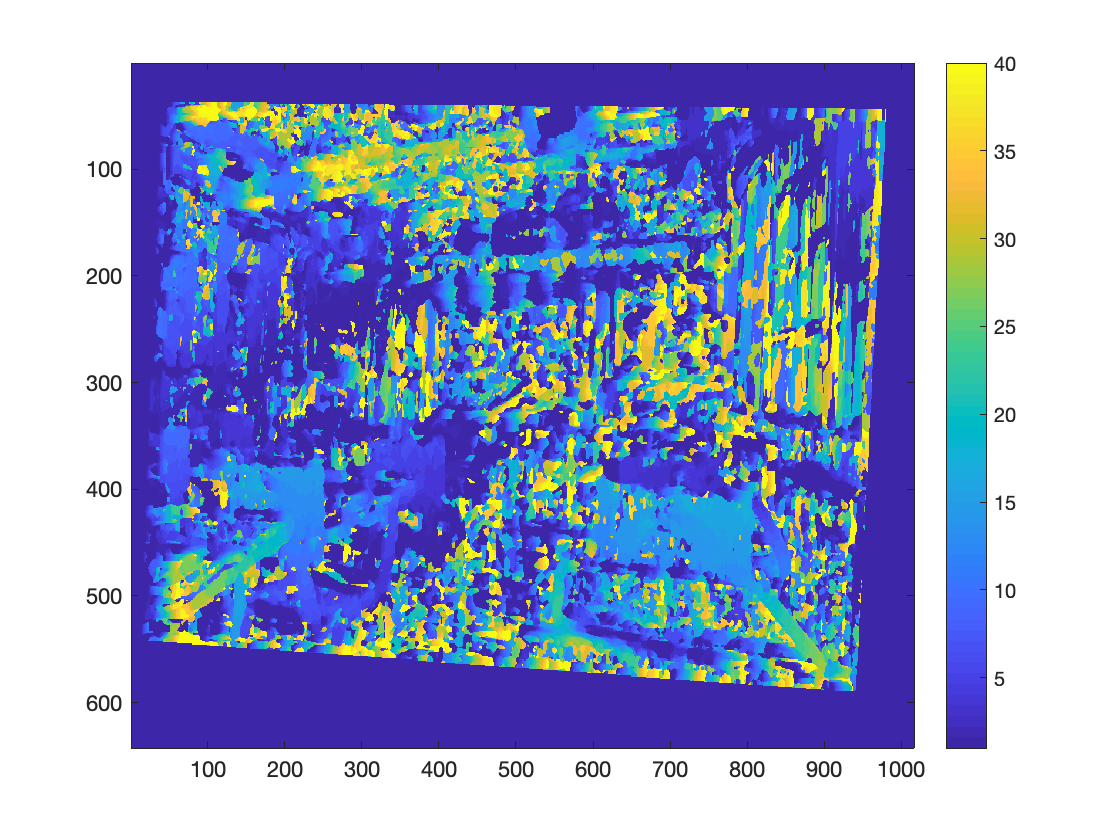
\includegraphics[width=0.4\textwidth]{../code/win9sig1.png} & 
	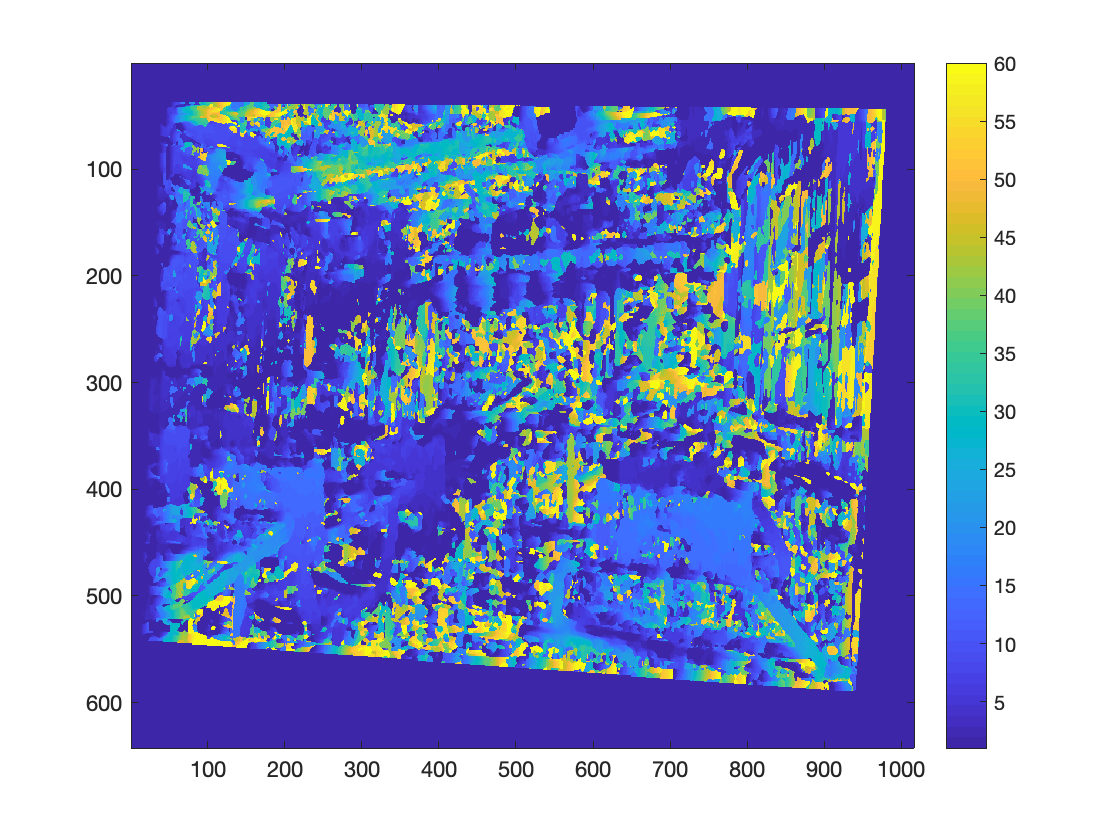
\includegraphics[width=0.4\textwidth]{../code/win9sig1disp60.png} \\
	\hline
	window size:9px, sigma:1, max\_disparity:40 &window size:9px, sigma:1, max\_disparity:60\\
	\hline
\end{longtable}

\end{document}